\documentclass[tikz,border=4pt]{standalone}
\usepackage{amsmath}
\begin{document}
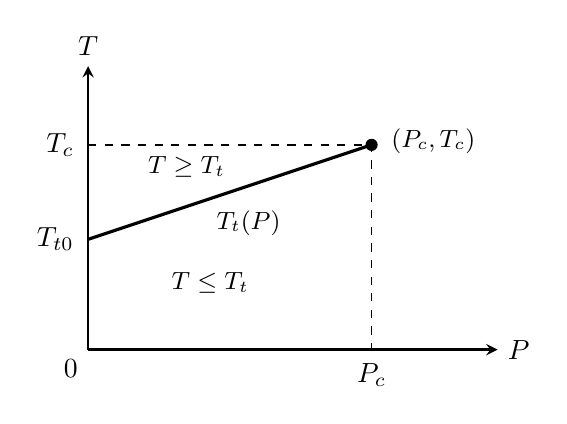
\begin{tikzpicture}[>=stealth, thick, scale=1.0]
  % Axes
  \draw[->, line width=0.8pt] (0, 0) -- (5.2, 0) node[right] {$P$};
  \draw[->, line width=0.8pt] (0, 0) -- (0, 3.6) node[above] {$T$};
  \node[below left] at (0, 0) {$0$};

  % First-order transition line T_t(P) from (0, 1.4) to critical point (3.6, 2.6)
  \draw[line width=1.15pt] (0, 1.4) -- (3.6, 2.6);
  \fill (3.6, 2.6) circle (2.2pt);

  % Dashed guides to axes
  \draw[dashed, line width=0.65pt] (0, 2.6) -- (3.6, 2.6) -- (3.6, 0);

  % Axis labels
  \node[left] at (-0.05, 1.4) {$T_{t0}$};
  \node[left] at (-0.05, 2.6) {$T_c$};
  \node[below] at (3.6, -0.05) {$P_c$};

  % Phase and curve labels
  \node[below right, font=\small] at (1.5, 1.9) {$T_t(P)$};
  \node[font=\small] at (1.25, 2.32) {$T \ge T_t$};
  \node[font=\small] at (1.55, 0.85) {$T \le T_t$};
  \node[right, font=\small] at (3.72, 2.65) {$(P_c, T_c)$};
\end{tikzpicture}
\end{document}
